\chapter{Results and Discussions}
\label{chap:results}

In the following, the results obtained from the finite element simulation using different setups are discussed and compared to the outer pressure field measurement.

\section{Comparison of simulation and measurement results}

\begin{figure}[H]
	\centering
	\begin{subfigure}[b]{0.49\textwidth}
		\centering
		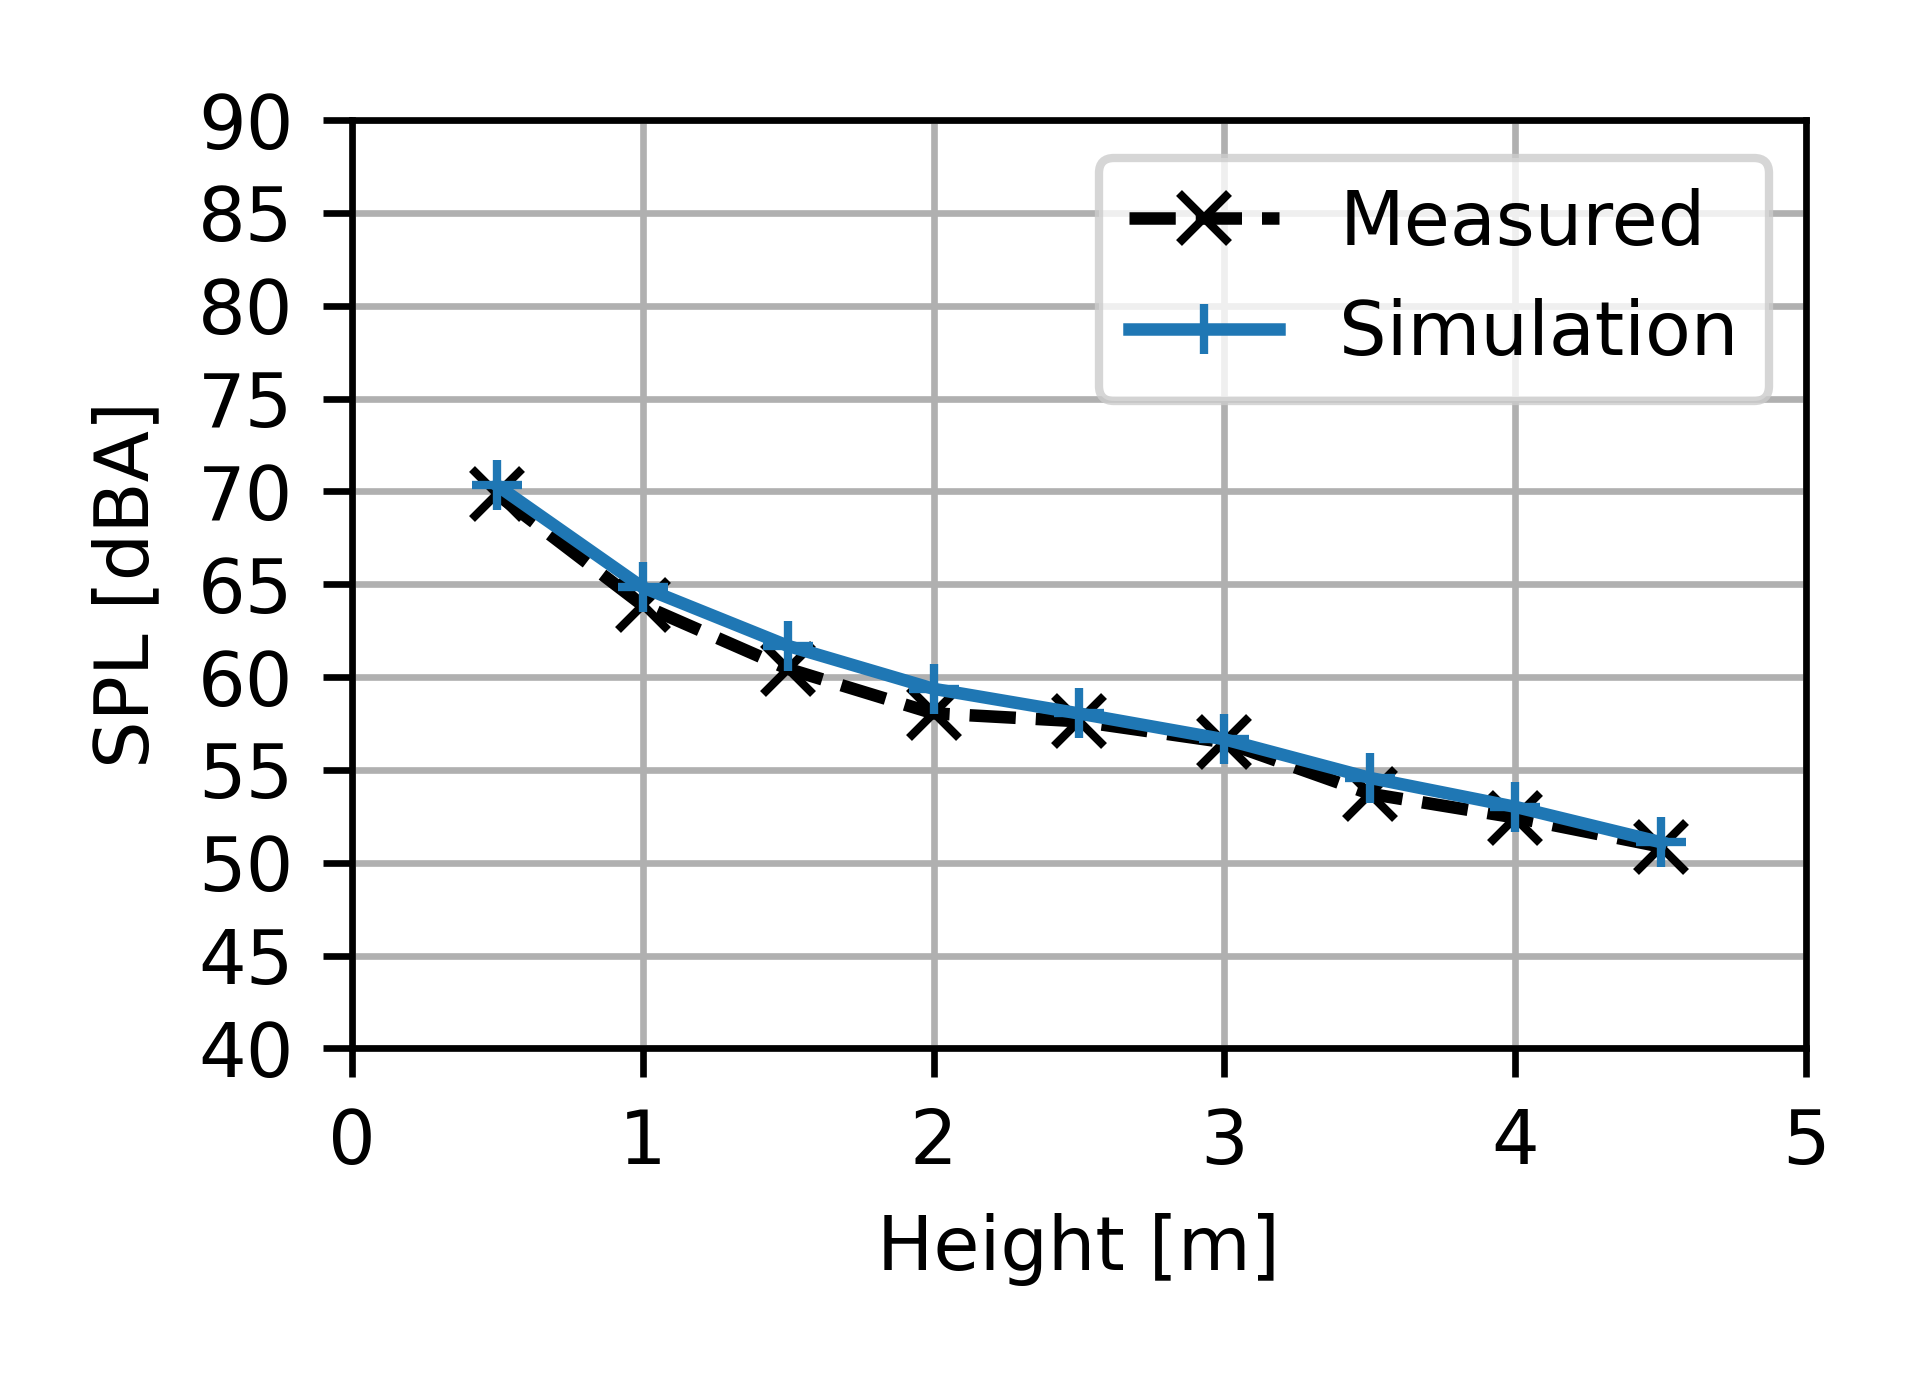
\includegraphics[width=\textwidth]{fig/chap5/initial_model/third_octave_over_height/125_Hz.png}
		\caption{125 Hz}
	\end{subfigure}
	\begin{subfigure}[b]{0.49\textwidth}
		\centering
		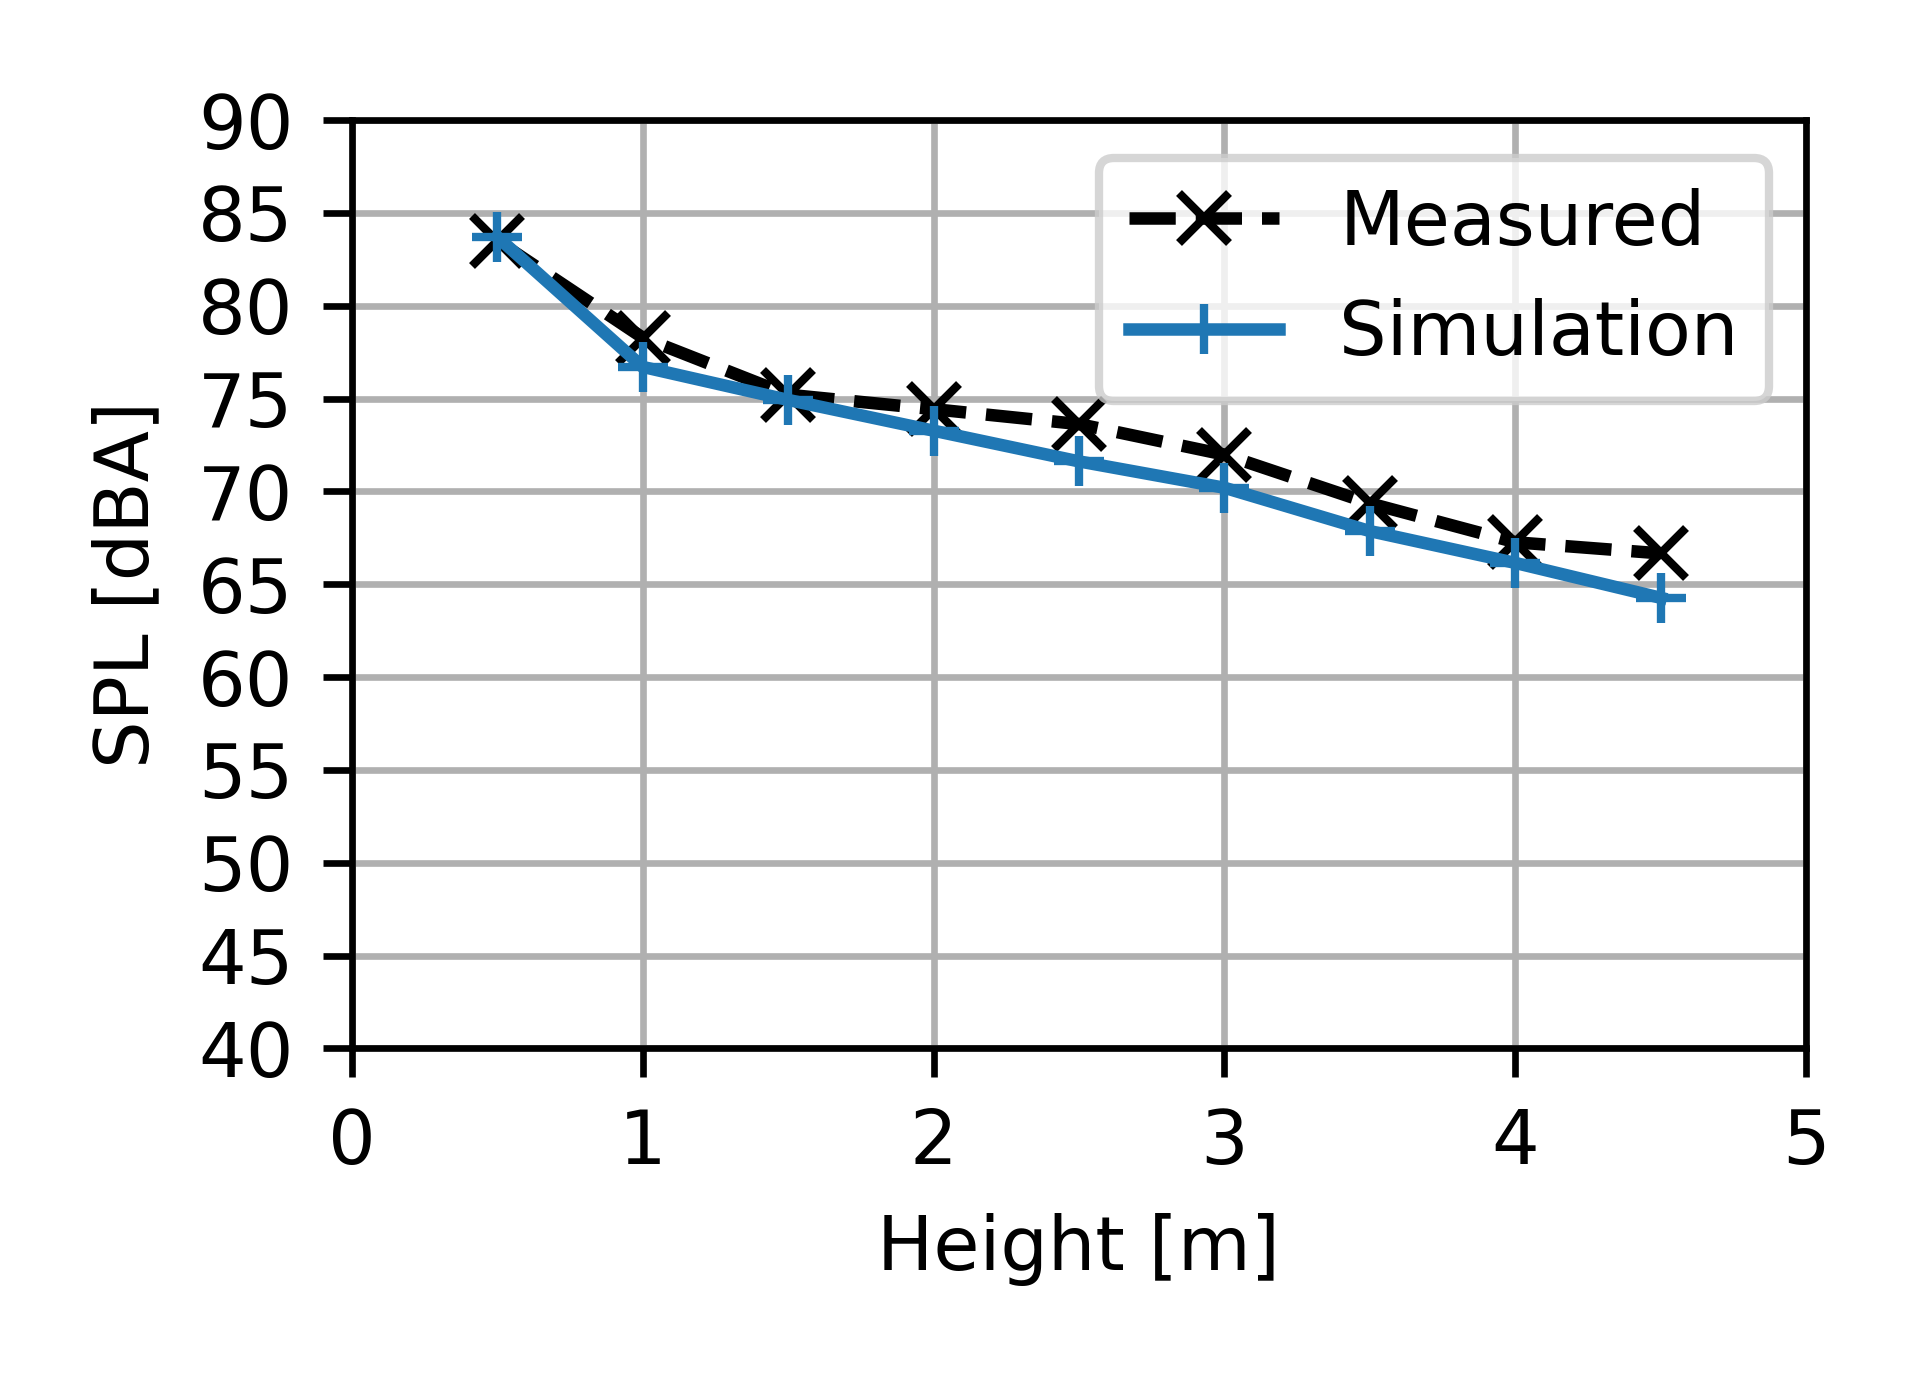
\includegraphics[width=\textwidth]{fig/chap5/initial_model/third_octave_over_height/400_Hz.png}
		\caption{400 Hz}
	\end{subfigure}
	\begin{subfigure}[b]{0.49\textwidth}
		\centering
		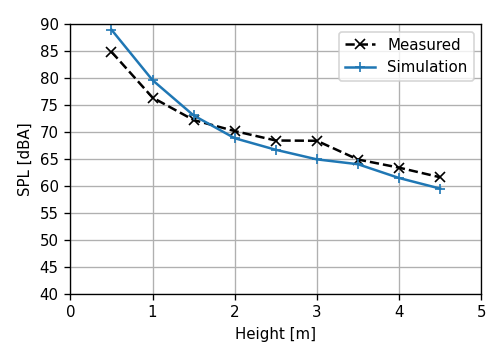
\includegraphics[width=\textwidth]{fig/chap5/initial_model/third_octave_over_height/1250_Hz.png}
		\caption{1250 Hz}
	\end{subfigure}
	\begin{subfigure}[b]{0.49\textwidth}
		\centering
		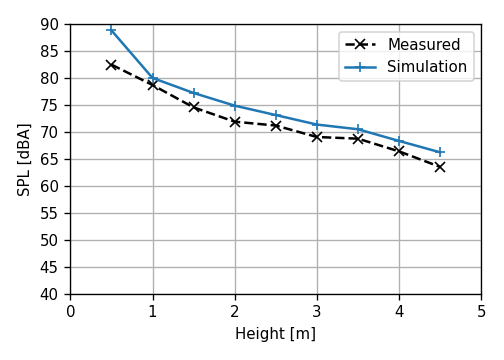
\includegraphics[width=\textwidth]{fig/chap5/initial_model/third_octave_over_height/2000_Hz.png}
		\caption{2000 Hz}
	\end{subfigure}
	\caption{Sound distribution at measurement position a, comparison between predictions obtained from the initial finite element model with the measurements. A-weighted SPL in one-third octave bands, dBA ref 20 $\mu$Pa.}
	\label{fig:third_octave_over_height}
\end{figure}

\begin{figure}[H]
	\centering
	\begin{subfigure}[b]{0.49\textwidth}
		\centering
		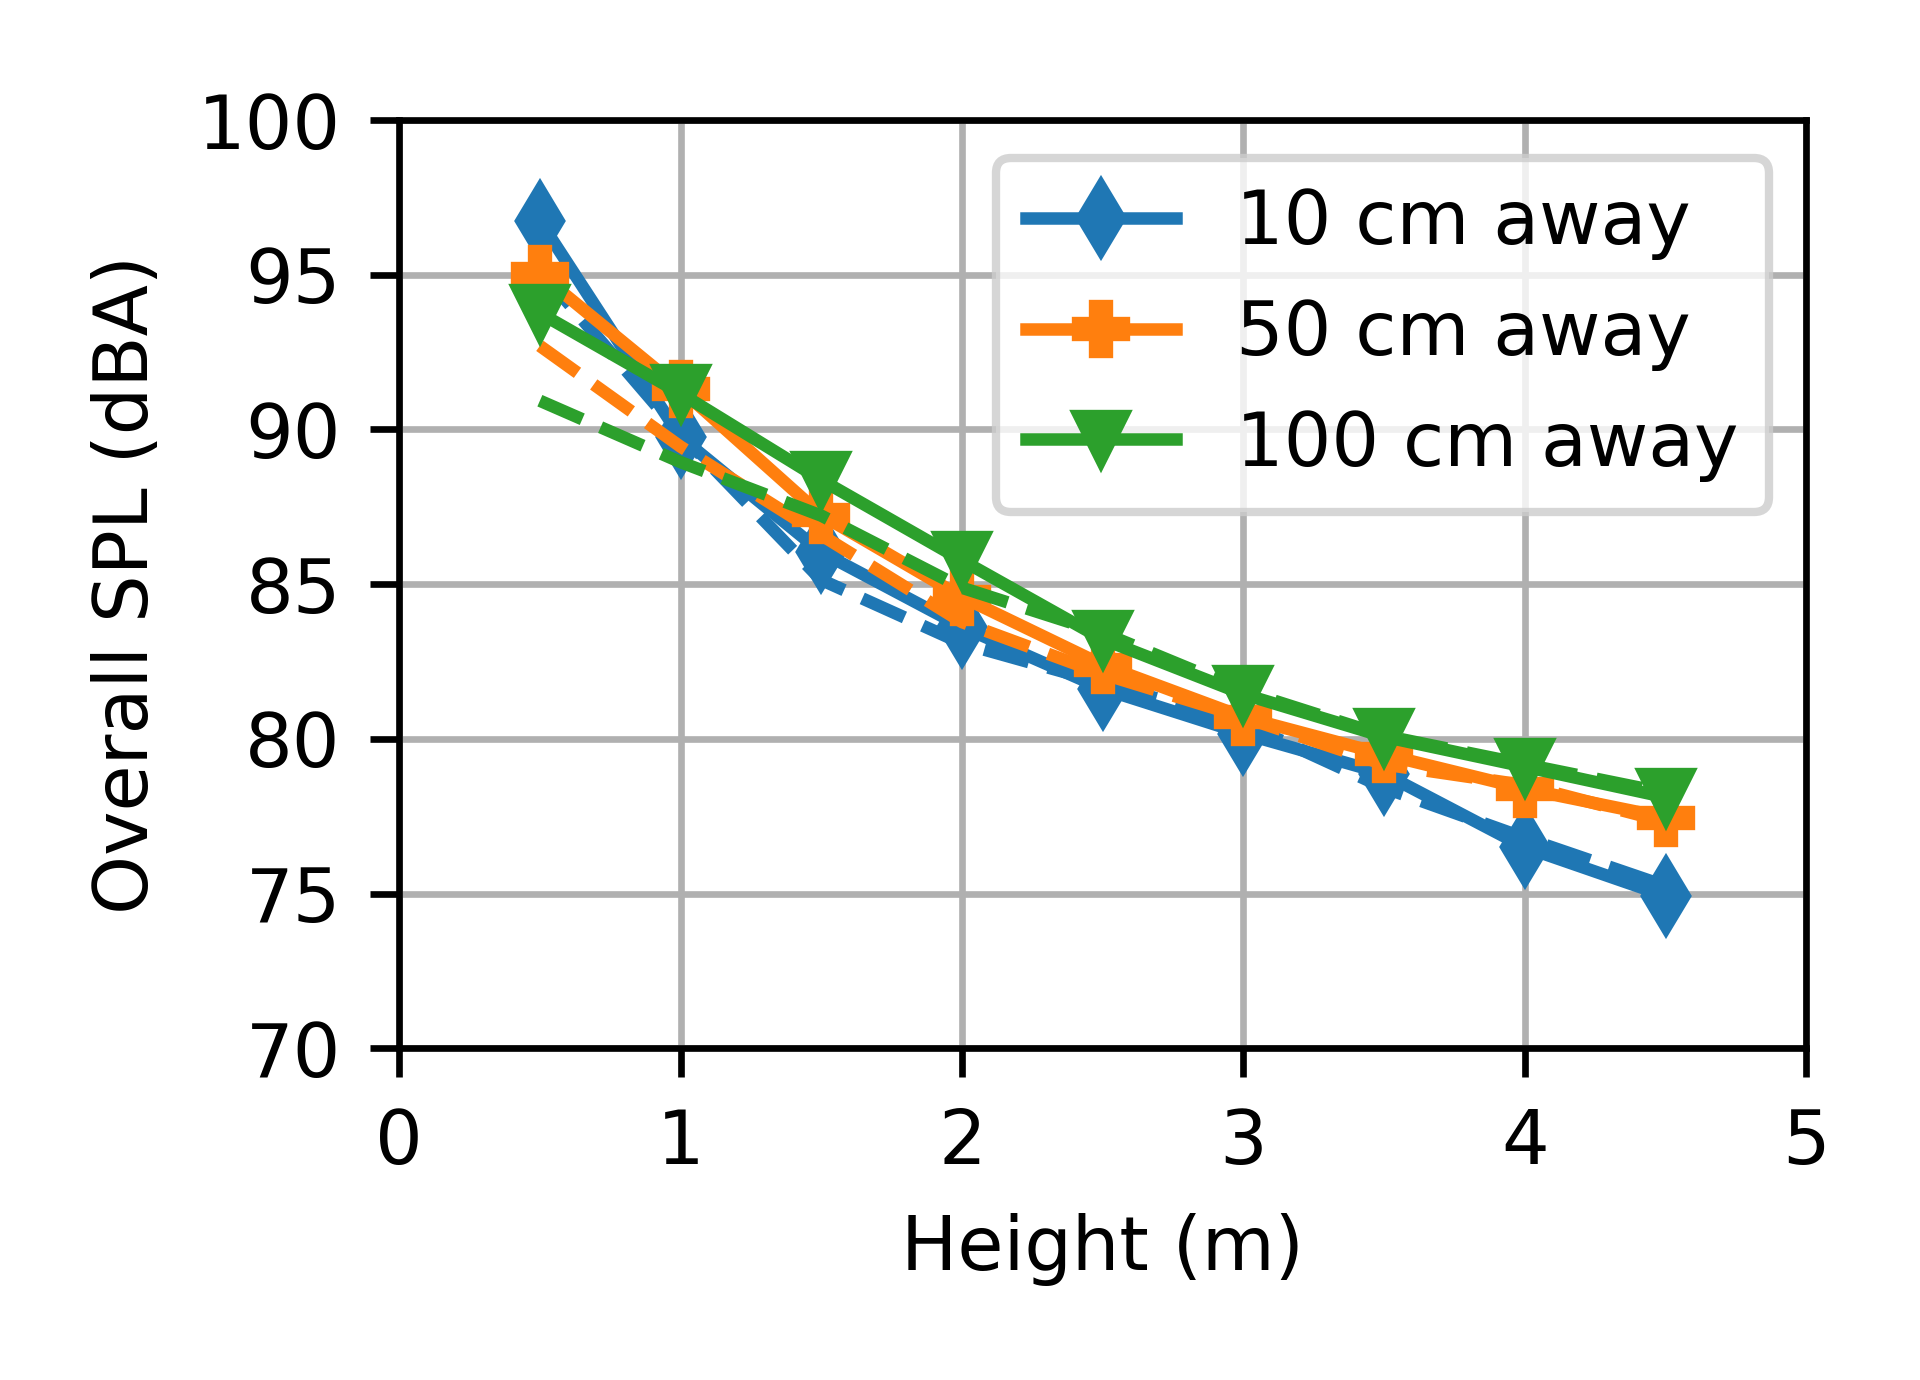
\includegraphics[width=\textwidth]{fig/chap5/initial_model/overall_SPL/all_pos.png}
		%\caption{2000 Hz}
	\end{subfigure}
	\begin{subfigure}[b]{0.49\textwidth}
		\centering
		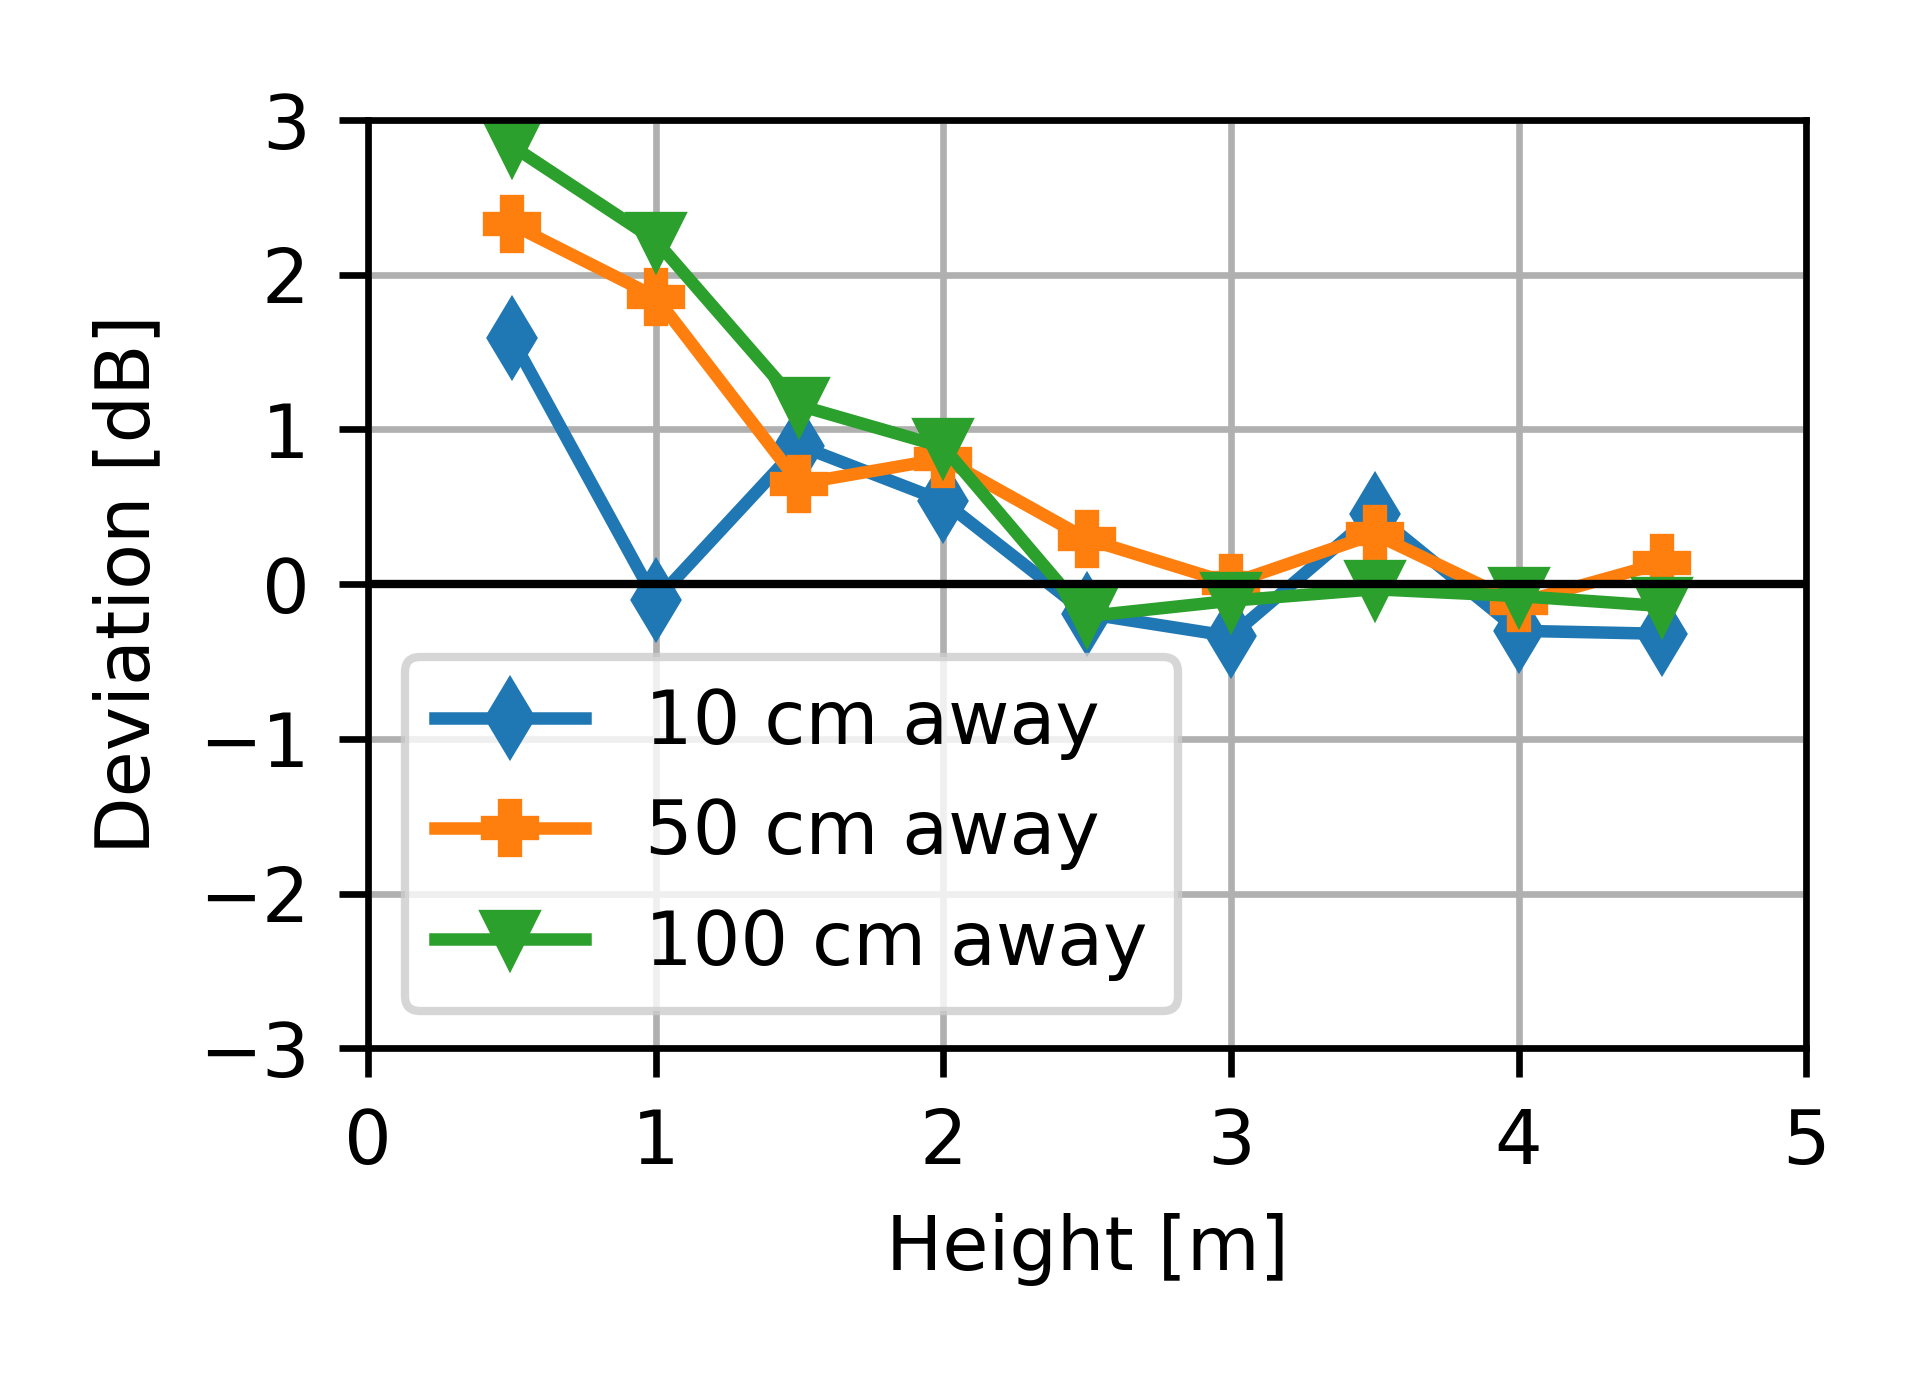
\includegraphics[width=\textwidth]{fig/chap5/initial_model/overall_SPL/deviation.png}
		%\caption{2000 Hz}
	\end{subfigure}
	\caption{Comparison of overall SPL in dBA ref 20 $\mu$Pa. Left: overall SPL as a function of height at various measurement positions (dashed curves: measurement; solid curves: simulation) Right: difference between simulation and measurement results}
	\label{fig:overall_SPL}
\end{figure}


\section{Effect of geometric variation}

\section{Effect of ground absorption}

\section{Effect of varing frequency steps per 1/3-octave band}